%% abtex2-modelo-trabalho-academico.tex, v-1.7.1 laurocesar
%% Copyright 2012-2013 by abnTeX2 group at http://abntex2.googlecode.com/ 
%%
%% This work may be distributed and/or modified under the
%% conditions of the LaTeX Project Public License, either version 1.3
%% of this license or (at your option) any later version.
%% The latest version of this license is in
%%   http://www.latex-project.org/lppl.txt
%% and version 1.3 or later is part of all distributions of LaTeX
%% version 2005/12/01 or later.
%%
%% This work has the LPPL maintenance status `maintained'.
%% 
%% The Current Maintainer of this work is the abnTeX2 team, led
%% by Lauro César Araujo. Further information are available on 
%% http://abntex2.googlecode.com/
%%
%% This work consists of the files abntex2-modelo-trabalho-academico.tex,
%% abntex2-modelo-include-comandos and abntex2-modelo-references.bib
%%

% ------------------------------------------------------------------------
% ------------------------------------------------------------------------
% abnTeX2: Modelo de Trabalho Academico (tese de doutorado, dissertacao de
% mestrado e trabalhos monograficos em geral) em conformidade com 
% ABNT NBR 14724:2011: Informacao e documentacao - Trabalhos academicos -
% Apresentacao
% ------------------------------------------------------------------------
% ------------------------------------------------------------------------


%%%%%%%%%%%%%%%%%%
%
% As alterações realizadas no leiaute original do abntex2 disponibilizado 
% no sharelatex adaptaram o leiaute do abntex2 aos requisitos mínimos
% para escrita de dissertações e teses customizadas para o 
% centro de informática da ufpe.
%
% Bruno Maciel <bifm@cin.ufpe.com> 20/10/2016
% Daniel Severo Estrázulas <dse@cin.ufpe.br> 19/10/2020
% Alterações realizadas para o template da biblioteca atualizado disponibilizado no site Versão 07.10.2020 (1.3) revisado pelas bibliotecárias do setor bibccen.pt@ufpe.br
%%%%%%%%%%%%%%%%%%%%%%%%%%%%%%%%%%%%%%%%%%%%%%%%%%%%%%%%%%%%%%%

\documentclass[
	% -- opções da classe memoir --
	12pt,				% tamanho da fonte
	openright,			% capítulos começam em pág ímpar (insere página vazia caso preciso)
	oneside,			% para impressão em verso e anverso. Oposto a oneside
	a4paper,			% tamanho do papel. 
	% -- opções da classe abntex2 --
	chapter=TITLE,		% títulos de capítulos convertidos em letras maiúsculas
	section=TITLE,		% títulos de seções convertidos em letras maiúsculas
	%subsection=TITLE,	% títulos de subseções convertidos em letras maiúsculas
	%subsubsection=TITLE,% títulos de subsubseções convertidos em letras maiúsculas
	% -- opções do pacote babel --
	%english,			% idioma adicional para hifenização
%	brazil,				% o último idioma é o principal do documento
	english,
	brazil,
	]{abntex2/abntex2}
	\renewcommand{\baselinestretch}{1.5} %para customizar o espaço entre as linhas do texto
% --
% SETTINGS

\usepackage{document\abntex2/abntex2-cin-ufpe}

% \usepackage[noframe]{showframe}
% \usepackage{showframe}

%\overfullrule=4mm %para identificar onde existem os alertas de linhas grandes mal formatada pelo LaTex, basta comentar para não aparecer a barra lateral preta na linha em questão.

\renewcommand*\arraystretch{1.2} %para customizar o espaço entre as linhas das tabelas


\usepackage{pdfpages} %para incluir pdf como páginas


% ---
% PACOTES
% ---
\usepackage{float}
\usepackage{cmap}				% Mapear caracteres especiais no PDF
\usepackage{lmodern}			% Usa a fonte Latin Modern			
\usepackage[T1]{fontenc}		% Selecao de codigos de fonte.
\usepackage[utf8]{inputenc}		% Codificacao do documento (conversão automática dos acentos)
\usepackage{lastpage}			% Usado pela Ficha catalográfica
\usepackage{indentfirst}		% Indenta o primeiro parágrafo de cada seção.
%\usepackage{color}				% Controle das cores
\usepackage{graphicx}			% Inclusão de gráficos
\usepackage{lipsum}				% para geração de dummy text
\usepackage[versalete,alf,abnt-and-type=e,abnt-etal-list=0,abnt-etal-cite=3]{abntex2/abntex2cite} 
\usepackage{multirow}
\usepackage[section]{placeins}



% -----------------------------------------------------------
% lista de abreviaturas e siglas
% início
% -----------------------------------------------------------
% \usepackage[noredefwarn,acronym]{glossaries} %GLOSSÁRIO
\usepackage[acronym,nonumberlist,nogroupskip,noredefwarn]{glossaries}
% \usepackage{glossary-superragged}

\newcolumntype{L}[1]{>{\raggedright\let\newline\\\arraybackslash\hspace{0pt}}m{#1}}
\newcolumntype{C}[1]{>{\centering\let\newline\\\arraybackslash\hspace{0pt}}m{#1}}
\newcolumntype{R}[1]{>{\raggedleft\let\newline\\\arraybackslash\hspace{0pt}}m{#1}}

\newglossarystyle{modsuper}{%
  \glossarystyle{super}%
  \renewcommand{\glsgroupskip}{}
  
  % put the glossary in a longtable environment:
 \renewenvironment{theglossary}%
  {
    \begin{longtable}
        {L{0.2\textwidth}L{0.8\textwidth}}}%
    {\end{longtable}
  }%
}

% -----------------------------------------------------------
% lista de abreviaturas e siglas
% fim
% -----------------------------------------------------------


\usepackage{lscape} 
\usepackage{rotating} %rotates the figures, page
\usepackage{tikz}
\usepackage[section]{placeins}
\usepackage{setspace} 



% ----------------------------------------------------------
% PERSONALIZAÇÃO DE CORES
% ----------------------------------------------------------
\definecolor{blue}{RGB}{41,5,195}
\definecolor{gray}{rgb}{.4,.4,.4}
\definecolor{gray}{rgb}{.4,.4,.4}
\definecolor{pblue}{rgb}{0.13,0.13,1}
\definecolor{pgreen}{rgb}{0,0.5,0}
\definecolor{pred}{rgb}{0.9,0,0}
\definecolor{pgrey}{rgb}{0.46,0.45,0.48}
\definecolor{lightgray}{rgb}{0.95, 0.95, 0.96}
\definecolor{whitesmoke}{rgb}{0.96, 0.96, 0.96}
\definecolor{javared}{rgb}{0.6,0,0} % for strings
\definecolor{javagreen}{rgb}{0.25,0.5,0.35} % comments
\definecolor{javapurple}{rgb}{0.5,0,0.35} % keywords
\definecolor{javadocblue}{rgb}{0.25,0.35,0.75} % javadoc
\definecolor{meucinza}{rgb}{0.5, 0.5, 0.5}
%\definecolor{lightgray}{gray}{0.9}


% ----------------------------------------------------------
% PERSONALIZAÇÃO DO USUÁRIO
% ----------------------------------------------------------

% ----------------------------------------------------------
% DADOS DO TRABALHO - CAPA e FOLHA DE ROSTO
% Configure os dados do trabalho aqui
% ----------------------------------------------------------


\titulo{\textbf{Análise de Dados Públicos da COVID-19 em Recife \\ Utilizando Aprendizagem de Máquina}}
\autor{JOÃO RAFAEL SANTOS CAMELO}
\local{Recife}
\data{\Year}
\orientador{\textbf{Orientador}: Fernando Maciano de Paula Neto}

\instituicao{UNIVERSIDADE FEDERAL DE PERNAMBUCO \\ CENTRO DE INFORMÁTICA \\ GRADUAÇÃO EM SISTEMAS DE INFORMAÇÃO}
\departamento{Centro de Informática}
\programa{Graduação em Sistemas de Informação}
\emailprograma{jrsc2@cin.ufpe.br}
\siteprograma{http://cin.ufpe.br/\textasciitilde posgraduacao}

\tipotrabalho{Trabalho de Graduação}
% O preambulo deve conter o tipo do trabalho, o objetivo, 
% o nome da instituição e a área de concentração 
%\preambulo{Trabalho apresentado ao Programa de Pós-graduação em Ciência da Computação do Centro de Informática da Universidade Federal de Pernambuco, como requisito parcial para obtenção do grau de Mestre Profissional em Ciência da Computação.}

%\preambuloatadefesa{Dissertação apresentada ao Programa de Pós-Graduação Profissional em Ciência da Computação da Universidade Federal de Pernambuco, como requisito parcial para a obtenção do título de Mestre Profissional em 04 de setembro de 2020.}

\preambulo{Trabalho apresentado ao Programa de Graduação em Sistemas de Informação do Centro de Informática da Universidade Federal de Pernambuco como requisito parcial para obtenção do grau de Bacharel em Sistemas de Informação}

\preambuloatadefesa{Monografia apresentada ao programa de Graduação em Sistemas de Informação do Centro de Informática da Universidade Federal de Pernambuco, sob o título Análise de Dados Públicos da COVID-19 em Recife Utilizando Aprendizagem de Máquina, orientada pelo Prof. Dr. Fernando Maciano de Paula Neto.}




\input{userlists}








% ----------------------------------------------------------
% COMPILA O ÍNDICE
% ----------------------------------------------------------
\makeindex
% ---


% ----------------------------------------------------------
% LISTA E ABREVIATURAS E SIGLAS
% ----------------------------------------------------------
%lista de siglas
\newacronym{MEC}{MEC}{Ministério da Educação}
\newacronym{UFPE}{UFPE}{Universidade Federal de Pernambuco}


\makenoidxglossaries
\renewcommand*{\glsseeformat}[3][\seename]{\textit{#1}  
\glsseelist{#2}}

\renewcommand*{\glspostdescription}{} % remove trailing dot
\renewcommand{\glsnamefont}[1]{\textbf{#1}}

\renewcommand{\familydefault}{\sfdefault}

% ----------------------------------------------------------
% GLOSSÁRIO
% ----------------------------------------------------------

\newglossaryentry{naive-bayes}
{
  name=\textit{Na{\"i}ve Bayes},
  description={},
  plural=\textit{Na{\"i}ve Bayes}
}

\newglossaryentry{hoeffding-tree}
{
  name=\textit{Hoeffding Tree},
  description={},
  plural=\textit{Hoeffding Trees}
}















\usepackage{pdfpages}
\usepackage{inconsolata}
\usepackage{listings}

\definecolor{cinza}{HTML}{FCF8F8}

% define formato e estilo dos elementos do tipo Codigo Fonte
\lstset{language=PHP,
basicstyle=\ttfamily\scriptsize,
%basicstyle=\ttfamily,
keywordstyle=\color{javapurple}\bfseries,
stringstyle=\color{pblue},
commentstyle=\color{javagreen},
morecomment=[s][\color{javadocblue}]{/**}{*/},
morecomment=[s][\color{gray}]{@}{\ },
numbers=left,
numberstyle=\tiny\color{black},
backgroundcolor=\color{cinza},
stepnumber=2,
numbersep=8pt,
xleftmargin=14pt,
tabsize=4,
showspaces=false,
showstringspaces=false,
breaklines=true,}

%%%%%%%%%%%%%%%%%%%%%%%%%%%%%%%%%%



\usepackage{adjustbox} % ajustar tabela ao tamanho da pagina


% ----------------------------------------------------------
% INÍCIO DO DOCUMENTO
% ----------------------------------------------------------
\begin{document}

\frenchspacing % Retira espaço extra obsoleto entre as frases.

\imprimircapa
\imprimirfolhaderosto*~
%a ficha deve ser passada pelo setor da biblioteca e sobrescrito no formato pdf

\includepdf[pages=-]{others/ficha.pdf}

%\newpage
% \input{document/others/ata_defesa}
%a folha de aprovação deve ser um pdf que a secretaria encaminha sem assinaturas
%basta fazer upload na basta others e sobrescrever

\includepdf[pages=-]{others/folha_aprovacao_original}

% ----------------------------------------------------------
% DEDICATÓRIA
% ----------------------------------------------------------
\begin{dedicatoria}
   \vspace*{\fill}
%   \centering
  % \noindent
   %\textit{\lipsum[2]} 
   Dedico este trabalho aos meus pais, sem os quais meus estudos não seriam possíveis.
   %\vspace*{\fill}
\end{dedicatoria}
% ---

% ----------------------------------------------------------
% AGRADECIMENTOS
% ----------------------------------------------------------
\begin{agradecimentos}
Aos meus pais, que com seu incentivo e apoio incondicional possibilitaram todas minhas conquistas presentes e futuras.

Ao meu orientador Fernando Maciano de Paula Neto, pelo suporte neste pouco tempo disponível, pelo seu direcionamento, correções e prontidão.

Aos amigos e companheiros de curso que fizeram parte da minha formação e que vão continuar presentes em minha vida.

À Prefeitura de Recife, pela disponibilização das estatísticas que foram de grande utilidade para a elaboração deste trabalho científico.

Aos profissionais de saúde, que serviram em linha de frente em momentos de crise.


\end{agradecimentos}


% ----------------------------------------------------------
% EPÍGRAFE

%Epígrafe: Elemento opcional e sem título em que o (a) autor (a) apresenta uma citação relacionada ao assunto tratado no trabalho. Deve ser elaborada conforme a ABNT-NBR 10520 (Citações). As citações de até três linhas devem estar entre aspas duplas e as citações com mais de três linhas devem ser destacadas com recuo de 4 cm da margem esquerda, com letra menor que a do texto e sem as aspas. A fonte da citação deve aparecer na lista de referências.
% ---------------------------------------------------------
\vspace*{10cm}

    \vspace*{10cm}
    
    
\begin{flushright}
\textit{Without data you're just another person with an opinion.}
\end{flushright}
\begin{flushright}
\vspace*{-0.3cm}
— William Edwards Deming
\end{flushright}
	
\newpage

% resumo em português
\begin{resumo}[Resumo] 
O combate à COVID-19 se tornou um grande desafio da saúde mundial, tendo mais de 22 milhões de casos e 615 mil mortes por todo o Brasil até a escrita deste trabalho. Em Recife, Pernambuco, até Setembro de 2021, mais de 600 mil casos foram documentados, onde mais de 7 mil resultaram na morte do paciente. Por meio da ampla coleta de dados realizada pela Prefeitura do Recife, este trabalho tem como objetivo comparar a efetividade de diferentes métodos de classificação por aprendizagem de máquina na análise de fatores de risco apresentados pela população, de forma a alertar para chances de casos graves da doença e possível óbito, se baseando nos dados demográficos e sintomáticos dos pacientes de Recife, assim como dados relativos à vacinação em progresso na cidade.
% \noindent %- o resumo deve ter apenas 1 parágrafo e sem recuo de texto na primeira linha, essa tag remove o recuo. Não pode haver quebra de linha.

 \vspace{\onelineskip}
    
 \noindent
 \textbf{Palavras-chaves}: Aprendizagem de máquina. COVID-19. Fatores de risco. Vacinação.
\end{resumo}



% resumo em inglês
\begin{resumo}[Abstract]
\begin{otherlanguage*}{english}

 %\noindent
Combating COVID-19 has become a major global health challenge, with more than 22 million cases and 615,000 deaths throughout Brazil as of the writing of this work. In Recife, Pernambuco, until September 2021, more than 600,000 cases were documented, where more than 7,000 resulted in the patient's death. Through the extensive data collection carried out by the City of Recife, this work aims to compare the effectiveness of different machine learning classification methods in the analysis of risk factors presented by the population, in order to alert to the chances of severe cases of the disease and possible death, based on demographic and symptomatic data of patients in Recife, as well as data on the ongoing vaccination in the city. 



   \vspace{\onelineskip} 
 
   \noindent 
   \textbf{Keywords}: COVID-19. Machine learning. Risk factors. Vaccination. 
 \end{otherlanguage*}
 \end{resumo}



% ----------------------------------------------------------
% LISTA DE FIGURAS
% ----------------------------------------------------------
\pdfbookmark[0]{\listfigurename}{lof}
\listoffigures*
\cleardoublepage


% ---
% LISTA DE CÓDIGOS FONTES
% ---

\pdfbookmark[0]{\lstlistingname}{lol} % caso não tenha quadros, comente esta linha 
\counterwithout{lstlisting}{chapter}



% Altera o nome padrão do rótulo usado no comando \autoref{}
\renewcommand{\lstlistingname}{Código Fonte}

% Altera o rótulo a ser usando no elemento pré-textual "Lista de código"
\renewcommand{\lstlistlistingname}{Lista de códigos}

% Configura a ``Lista de Códigos'' conforme as regras da ABNT (para abnTeX2)
\begingroup\makeatletter
\let\newcounter\@gobble\let\setcounter\@gobbletwo
  \globaldefs\@ne \let\c@loldepth\@ne
  \newlistof{listings}{lol}{\lstlistlistingname}
  \newlistentry{lstlisting}{lol}{0}
\endgroup

\renewcommand{\cftlstlistingaftersnum}{\hfill--\hfil}

\let\oldlstlistoflistings\lstlistoflistings
{
\let\oldnumberline\numberline
\newcommand{\algnumberline}[1]{Código Fonte~#1~\enspace--~\enspace}
\renewcommand{\numberline}{\algnumberline}

\begin{KeepFromToc}
\lstlistoflistings
\end{KeepFromToc}
}
\cleardoublepage

% ---
% LISTA DE QUADROS
% ---
\pdfbookmark[0]{\listofquadrosname}{loq} % caso não tenha quadros, comente esta linha 
\listofquadros* % caso não tenha quadros, comente esta linha 
\cleardoublepage



% ----------------------------------------------------------
% LISTA DE TABELAS
% ----------------------------------------------------------

\pdfbookmark[0]{\listtablename}{lot}
\listoftables*
\cleardoublepage


        
  
% ----------------------------------------------------------
% LISTA E ABREVIATURAS E SIGLAS
% ----------------------------------------------------------
% \printglossary[type=\acronymtype,title={\listadesiglasname},nonumberlist]
% \printglossaries
% compile uma vez com o comando \printglossaries e depois compile novamente com o comando \printglossaries comentado para as páginas glossário e siglas serem ocultadas.

% ----------------------------------------------------------
% LISTA E ABREVIATURAS E SIGLAS
% ----------------------------------------------------------
% \setglossarystyle{modsuper}
\printnoidxglossary[style=modsuper,type=\acronymtype,title={\listadesiglasname},nonumberlist]
% \printglossary[style=super, type=\acronymtype]
\cleardoublepage



% ----------------------------------------------------------
% LISTA DE SIMBOLOS
% ----------------------------------------------------------



% ---

% ---
% inserir lista de símbolos
% ---
\begin{simbolos}
  \item[$ \gamma $] Letra grega Gama
  %\item[$ \Lambda $] Lambda
  %\item[$ \zeta $] Letra grega minúscula zeta
  \item[$ \in $] Pertence
%  \item[$ \infty$] Infinito
%  \item[$ \ge$] Maior ou Igual
  \item[$ \delta$] Delta
  \item[$ \theta$] Teta
  \item[$ \sigma$] Sigma
  \item[$ \mu$] Mi
  
\end{simbolos}
% ---




% ----------------------------------------------------------
%


% ---

% ---
% inserir lista de símbolos
% ---
\begin{simbolos}
  \item[$ \gamma $] Letra grega Gama
  %\item[$ \Lambda $] Lambda
  %\item[$ \zeta $] Letra grega minúscula zeta
  \item[$ \in $] Pertence
%  \item[$ \infty$] Infinito
%  \item[$ \ge$] Maior ou Igual
  \item[$ \delta$] Delta
  \item[$ \theta$] Teta
  \item[$ \sigma$] Sigma
  \item[$ \mu$] Mi
  
\end{simbolos}
% ---






% ----------------------------------------------------------
% SUMÁRIO
% ----------------------------------------------------------
\pdfbookmark[0]{\contentsname}{toc}
\tableofcontents*
% \begingroup\intoctrue
% \tableofcontents*
% \endgroup
\cleardoublepage

% \setcounter{page}{13}
\setcounter{tocdepth}{2}
\setcounter{table}{0}




% ----------------------------------------------------------
% ELEMENTOS TEXTUAIS
% ----------------------------------------------------------
\textual


% referencie todos os arquivos de capítulos aqui, fique a vontade para
% fazer a sua organização de diretórios

  \chapter{Introdução}
\label{chap:intro}

\section{Motivação}
\label{motivacao}

Texto texto texto texto texto texto texto texto texto texto texto texto texto texto texto texto texto texto texto texto texto texto texto texto texto texto texto texto texto texto texto texto texto texto texto texto, \textbf{exemplo} sigla \gls{UFPE}.

\input{images/captitulo1/figuraex}

Texto texto texto texto texto texto texto texto texto texto texto texto texto texto texto texto texto texto texto texto texto texto texto texto texto texto texto texto texto texto texto texto texto texto texto texto, conforme Figuras \ref{fig:figuraex} e Figuras \ref{fig:figuraex2}, continua no Capítulo \ref{chap:outrocapitulo}.


\input{images/captitulo1/figuraex2}

Texto texto texto texto texto texto texto texto texto texto texto texto texto texto texto texto texto texto texto texto texto texto texto texto texto texto texto \gls{UFPE}.


\section{Objetivos}
\label{sec:objetivos}

\subsection{Gerais}
\label{subsec:objetivosgerais}

Este trabalho tem como objetivo geral avaliar a eficácia de diferentes algoritmos de classificação por aprendizagem de máquina na identificação de variáveis que refletem em uma maior chance de casos de COVID-19 alcançarem uma severidade grave ou resultarem em óbito, utilizando dados demográficos, sintomáticos, e o progresso da vacinação na cidade do Recife.

\subsection{Específicos}
\label{subsec:objetivosespecificos}

\begin{itemize}
  \item Aplicar algoritmos de classificação por aprendizagem de máquina nas bases de dados disponibilizadas pela Prefeitura do Recife;
  \item Analisar os resultados e comparar a eficácia dos métodos implementados;
  \item Identificar fatores de risco e sintomas apresentados, de forma a auxiliar na tomada de decisão do tratamento dos pacientes;
  \item Verificar o impacto da vacinação em progresso nos fatores de risco identificados.
\end{itemize}

  \chapter{Introdução}
\label{chap:intro}

\section{Motivação}
\label{motivacao}

Texto texto texto texto texto texto texto texto texto texto texto texto texto texto texto texto texto texto texto texto texto texto texto texto texto texto texto texto texto texto texto texto texto texto texto texto, \textbf{exemplo} sigla \gls{UFPE}.

\input{images/captitulo1/figuraex}

Texto texto texto texto texto texto texto texto texto texto texto texto texto texto texto texto texto texto texto texto texto texto texto texto texto texto texto texto texto texto texto texto texto texto texto texto, conforme Figuras \ref{fig:figuraex} e Figuras \ref{fig:figuraex2}, continua no Capítulo \ref{chap:outrocapitulo}.


\input{images/captitulo1/figuraex2}

Texto texto texto texto texto texto texto texto texto texto texto texto texto texto texto texto texto texto texto texto texto texto texto texto texto texto texto \gls{UFPE}.


\section{Objetivos}
\label{sec:objetivos}

\subsection{Gerais}
\label{subsec:objetivosgerais}

Este trabalho tem como objetivo geral avaliar a eficácia de diferentes algoritmos de classificação por aprendizagem de máquina na identificação de variáveis que refletem em uma maior chance de casos de COVID-19 alcançarem uma severidade grave ou resultarem em óbito, utilizando dados demográficos, sintomáticos, e o progresso da vacinação na cidade do Recife.

\subsection{Específicos}
\label{subsec:objetivosespecificos}

\begin{itemize}
  \item Aplicar algoritmos de classificação por aprendizagem de máquina nas bases de dados disponibilizadas pela Prefeitura do Recife;
  \item Analisar os resultados e comparar a eficácia dos métodos implementados;
  \item Identificar fatores de risco e sintomas apresentados, de forma a auxiliar na tomada de decisão do tratamento dos pacientes;
  \item Verificar o impacto da vacinação em progresso nos fatores de risco identificados.
\end{itemize}
  
  \chapter{Introdução}
\label{chap:intro}

\section{Motivação}
\label{motivacao}

Texto texto texto texto texto texto texto texto texto texto texto texto texto texto texto texto texto texto texto texto texto texto texto texto texto texto texto texto texto texto texto texto texto texto texto texto, \textbf{exemplo} sigla \gls{UFPE}.

\input{images/captitulo1/figuraex}

Texto texto texto texto texto texto texto texto texto texto texto texto texto texto texto texto texto texto texto texto texto texto texto texto texto texto texto texto texto texto texto texto texto texto texto texto, conforme Figuras \ref{fig:figuraex} e Figuras \ref{fig:figuraex2}, continua no Capítulo \ref{chap:outrocapitulo}.


\input{images/captitulo1/figuraex2}

Texto texto texto texto texto texto texto texto texto texto texto texto texto texto texto texto texto texto texto texto texto texto texto texto texto texto texto \gls{UFPE}.


\section{Objetivos}
\label{sec:objetivos}

\subsection{Gerais}
\label{subsec:objetivosgerais}

Este trabalho tem como objetivo geral avaliar a eficácia de diferentes algoritmos de classificação por aprendizagem de máquina na identificação de variáveis que refletem em uma maior chance de casos de COVID-19 alcançarem uma severidade grave ou resultarem em óbito, utilizando dados demográficos, sintomáticos, e o progresso da vacinação na cidade do Recife.

\subsection{Específicos}
\label{subsec:objetivosespecificos}

\begin{itemize}
  \item Aplicar algoritmos de classificação por aprendizagem de máquina nas bases de dados disponibilizadas pela Prefeitura do Recife;
  \item Analisar os resultados e comparar a eficácia dos métodos implementados;
  \item Identificar fatores de risco e sintomas apresentados, de forma a auxiliar na tomada de decisão do tratamento dos pacientes;
  \item Verificar o impacto da vacinação em progresso nos fatores de risco identificados.
\end{itemize}

  \chapter{Introdução}
\label{chap:intro}

\section{Motivação}
\label{motivacao}

Texto texto texto texto texto texto texto texto texto texto texto texto texto texto texto texto texto texto texto texto texto texto texto texto texto texto texto texto texto texto texto texto texto texto texto texto, \textbf{exemplo} sigla \gls{UFPE}.

\input{images/captitulo1/figuraex}

Texto texto texto texto texto texto texto texto texto texto texto texto texto texto texto texto texto texto texto texto texto texto texto texto texto texto texto texto texto texto texto texto texto texto texto texto, conforme Figuras \ref{fig:figuraex} e Figuras \ref{fig:figuraex2}, continua no Capítulo \ref{chap:outrocapitulo}.


\input{images/captitulo1/figuraex2}

Texto texto texto texto texto texto texto texto texto texto texto texto texto texto texto texto texto texto texto texto texto texto texto texto texto texto texto \gls{UFPE}.


\section{Objetivos}
\label{sec:objetivos}

\subsection{Gerais}
\label{subsec:objetivosgerais}

Este trabalho tem como objetivo geral avaliar a eficácia de diferentes algoritmos de classificação por aprendizagem de máquina na identificação de variáveis que refletem em uma maior chance de casos de COVID-19 alcançarem uma severidade grave ou resultarem em óbito, utilizando dados demográficos, sintomáticos, e o progresso da vacinação na cidade do Recife.

\subsection{Específicos}
\label{subsec:objetivosespecificos}

\begin{itemize}
  \item Aplicar algoritmos de classificação por aprendizagem de máquina nas bases de dados disponibilizadas pela Prefeitura do Recife;
  \item Analisar os resultados e comparar a eficácia dos métodos implementados;
  \item Identificar fatores de risco e sintomas apresentados, de forma a auxiliar na tomada de decisão do tratamento dos pacientes;
  \item Verificar o impacto da vacinação em progresso nos fatores de risco identificados.
\end{itemize}

  \chapter{Introdução}
\label{chap:intro}

\section{Motivação}
\label{motivacao}

Texto texto texto texto texto texto texto texto texto texto texto texto texto texto texto texto texto texto texto texto texto texto texto texto texto texto texto texto texto texto texto texto texto texto texto texto, \textbf{exemplo} sigla \gls{UFPE}.

\input{images/captitulo1/figuraex}

Texto texto texto texto texto texto texto texto texto texto texto texto texto texto texto texto texto texto texto texto texto texto texto texto texto texto texto texto texto texto texto texto texto texto texto texto, conforme Figuras \ref{fig:figuraex} e Figuras \ref{fig:figuraex2}, continua no Capítulo \ref{chap:outrocapitulo}.


\input{images/captitulo1/figuraex2}

Texto texto texto texto texto texto texto texto texto texto texto texto texto texto texto texto texto texto texto texto texto texto texto texto texto texto texto \gls{UFPE}.


\section{Objetivos}
\label{sec:objetivos}

\subsection{Gerais}
\label{subsec:objetivosgerais}

Este trabalho tem como objetivo geral avaliar a eficácia de diferentes algoritmos de classificação por aprendizagem de máquina na identificação de variáveis que refletem em uma maior chance de casos de COVID-19 alcançarem uma severidade grave ou resultarem em óbito, utilizando dados demográficos, sintomáticos, e o progresso da vacinação na cidade do Recife.

\subsection{Específicos}
\label{subsec:objetivosespecificos}

\begin{itemize}
  \item Aplicar algoritmos de classificação por aprendizagem de máquina nas bases de dados disponibilizadas pela Prefeitura do Recife;
  \item Analisar os resultados e comparar a eficácia dos métodos implementados;
  \item Identificar fatores de risco e sintomas apresentados, de forma a auxiliar na tomada de decisão do tratamento dos pacientes;
  \item Verificar o impacto da vacinação em progresso nos fatores de risco identificados.
\end{itemize}

\bookmarksetup{startatroot}% 


% ----------------------------------------------------------
% ELEMENTOS PÓS-TEXTUAIS
% ----------------------------------------------------------
\postextual


% ----------------------------------------------------------
% Referências bibliográficas
% ----------------------------------------------------------
%\bibliographystyle{abntexalfenglish} %caso seja em inglês, retire o comentário desta linha

% \renewcommand{\bibname}{REFER\^ENCIAS}
%\renewcommand{\bibname}{Bibliography}
% \addbibresource{sample.bib}
\bibliography{references2}


% ----------------------------------------------------------
% Apêndices
% ----------------------------------------------------------


% ----------------------
% força para que não exiba subtítulos em apêndices no sumário
% -----------------------

\begin{apendicesenv}
\addtocontents{toc}{\protect\setcounter{tocdepth}{1}}
\makeatletter
\addtocontents{toc}{%
  \begingroup
  \let\protect\l@chapter\protect\l@section
  \let\protect\l@section\protect\l@subsection
}
\makeatother

% Imprime uma página indicando o início dos apêndices
% \partapendices

%coloca o identificador do anexo/apendice somente na primeira página
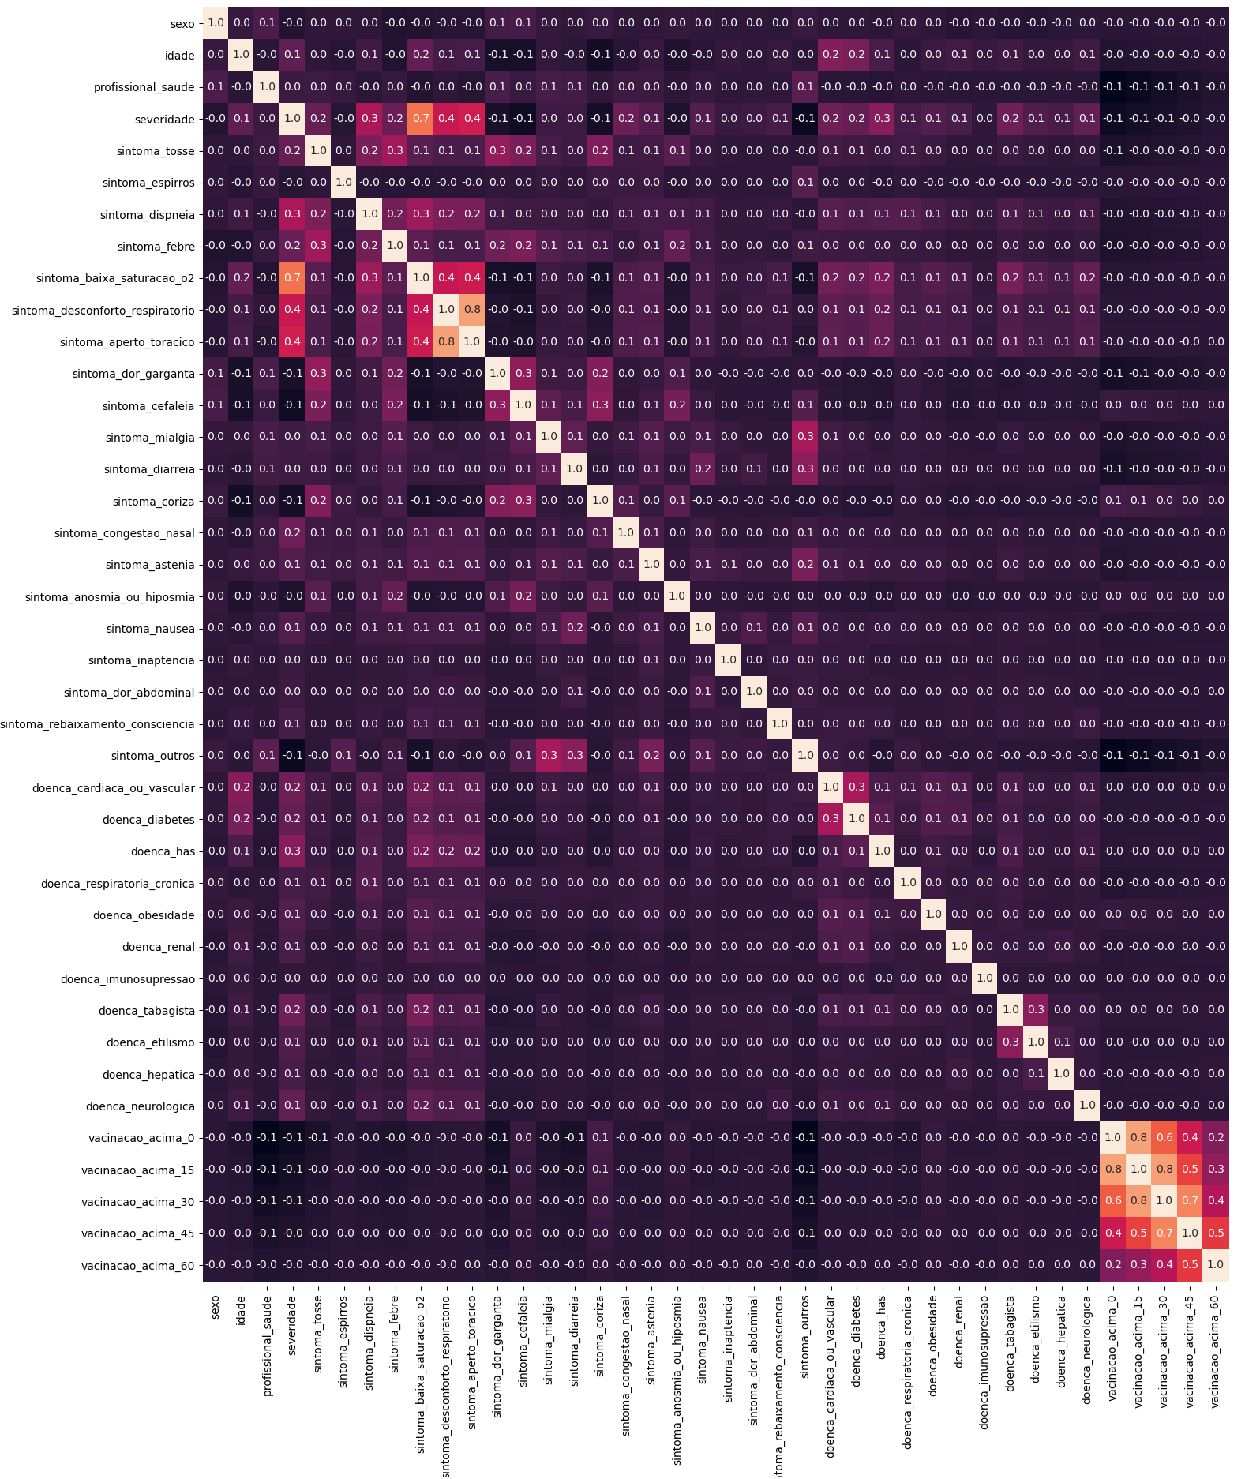
\includepdf[pages={1},scale=0.8,pagecommand=\chapter{Mapa de Calor de Correlação}\label{apendice:correlacao}]{appendix/correlation}

%coloca o identificador do anexo/apendice somente na primeira página
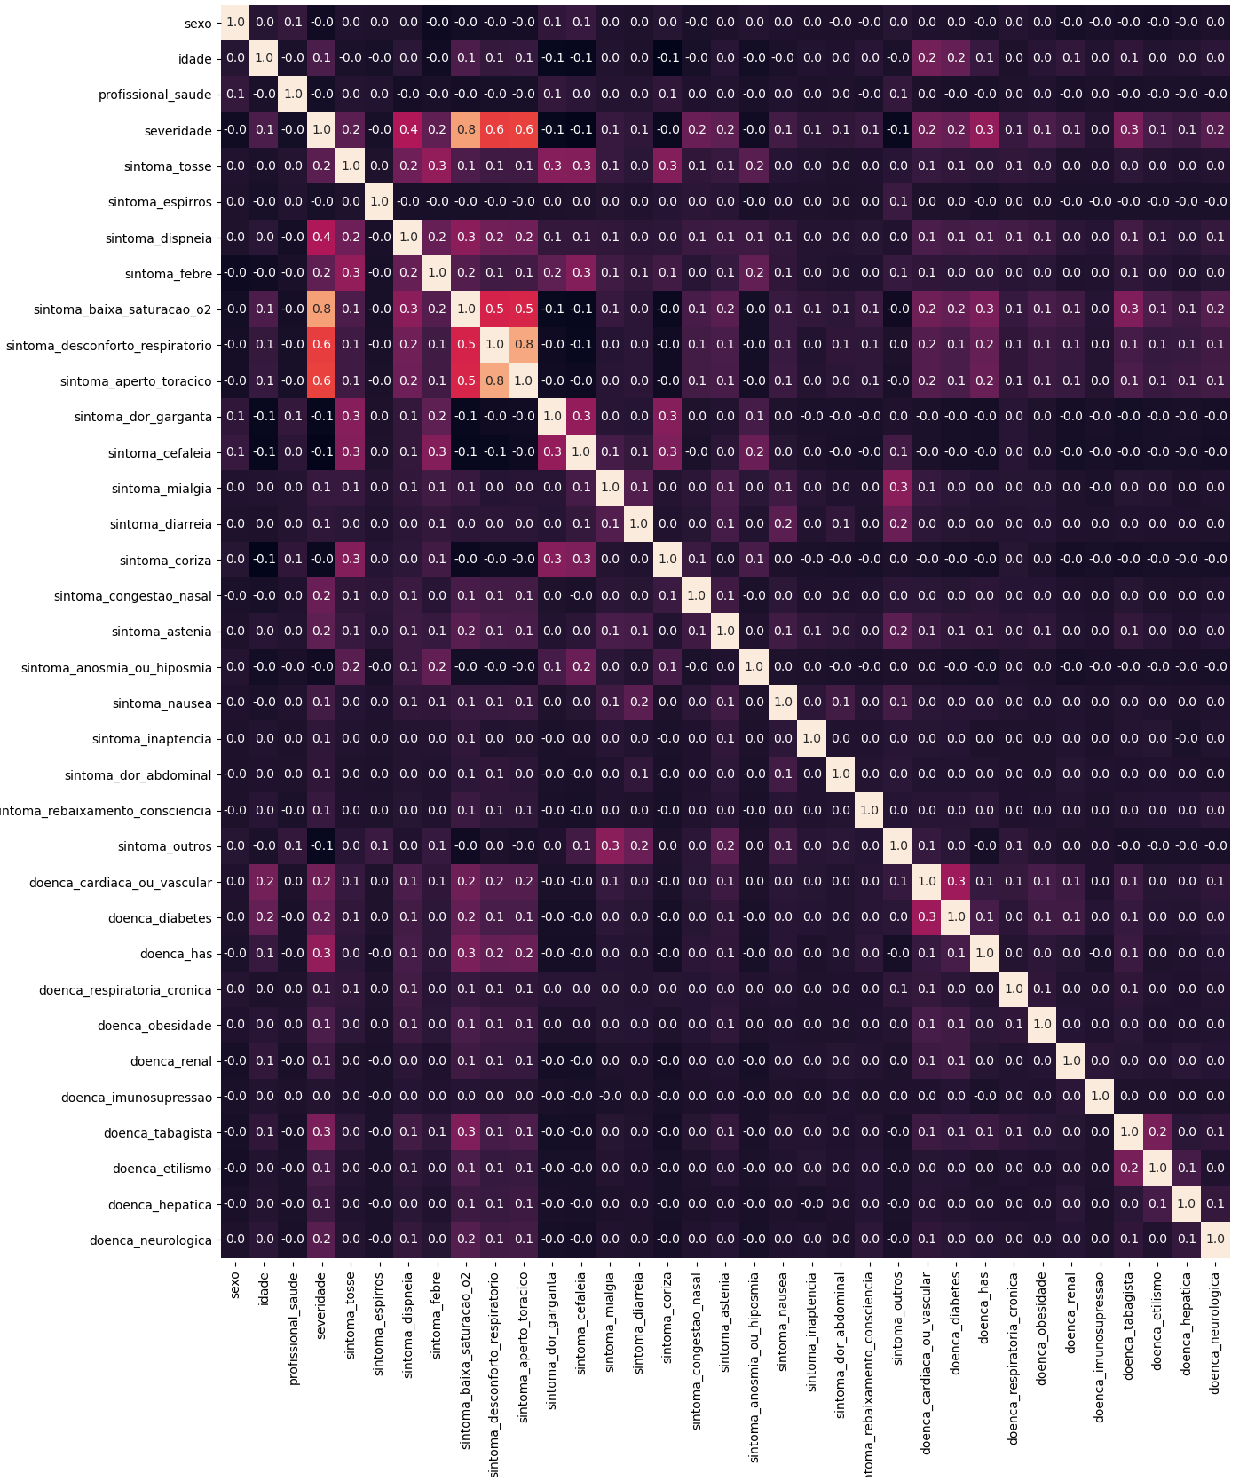
\includepdf[pages={1},scale=0.8,pagecommand=\chapter{Mapa de Calor de Correlação Antes da Vacinação}\label{apendice:correlacao-v0}]{appendix/correlation-v0}

%coloca o identificador do anexo/apendice somente na primeira página
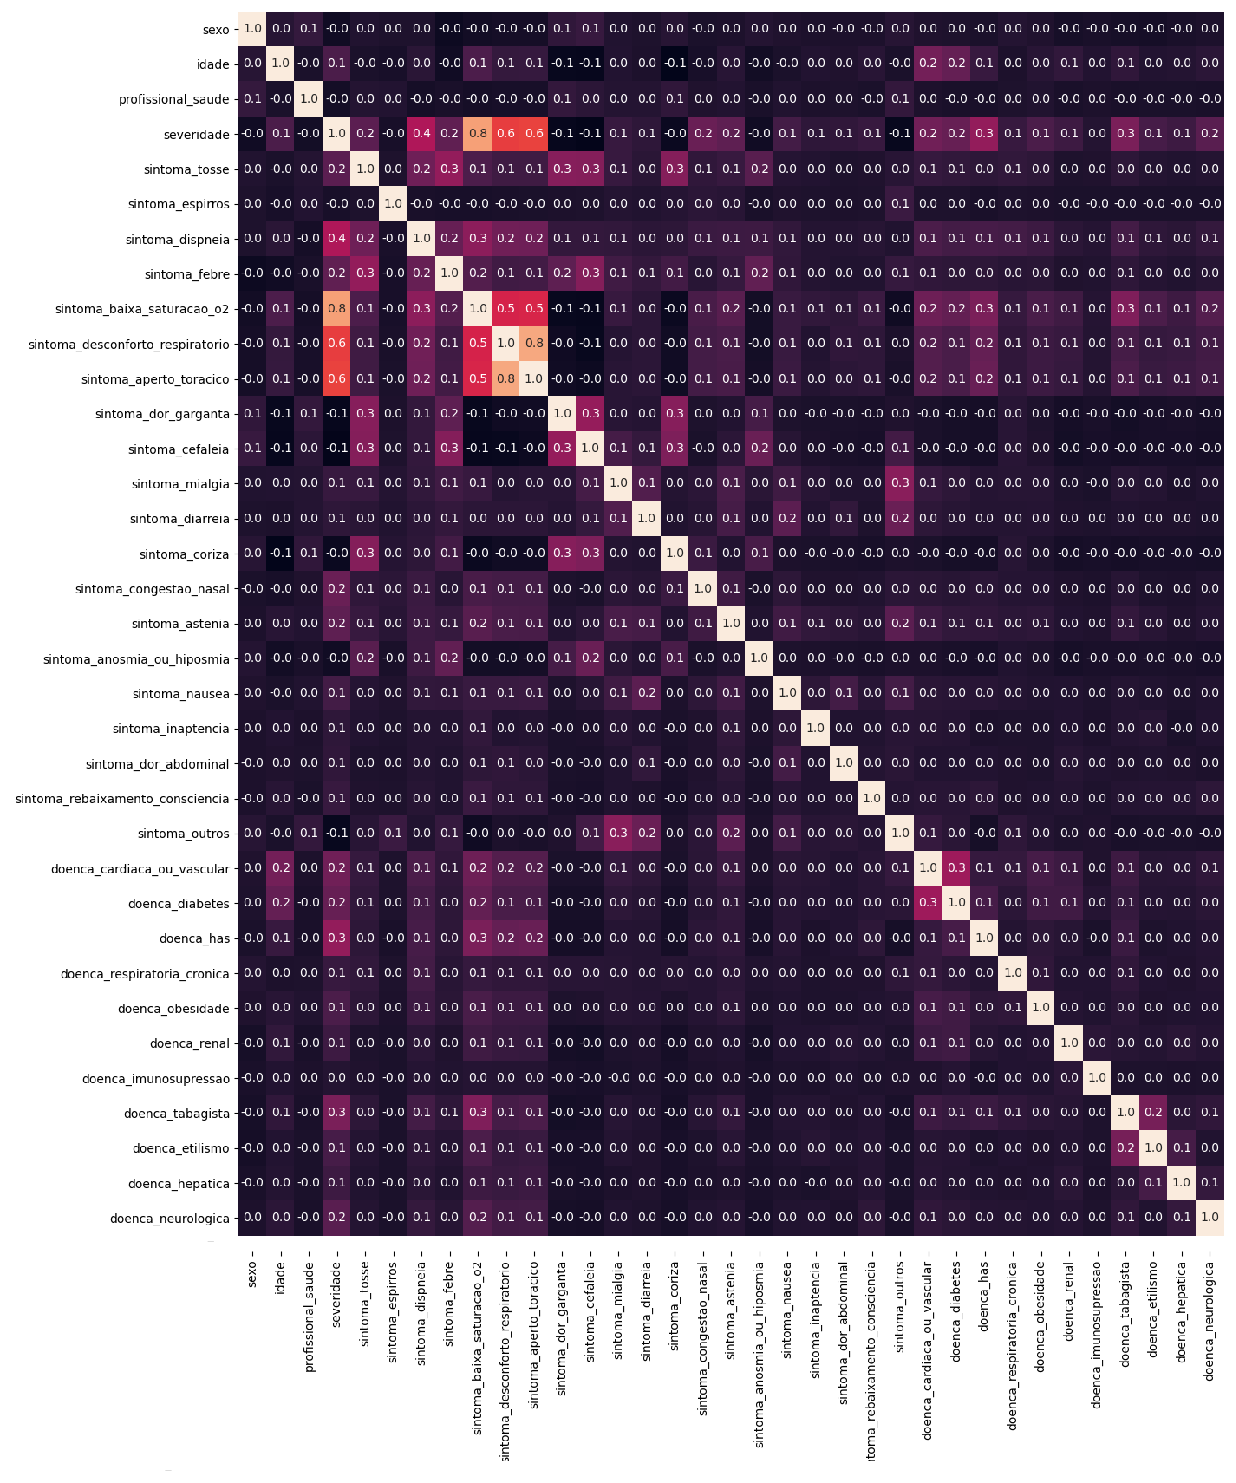
\includepdf[pages={1},scale=0.8,pagecommand=\chapter{Mapa de Calor de Correlação com 30\% de Vacinação}\label{apendice:correlacao-v30}]{appendix/correlation-v30}


\addtocontents{toc}{\endgroup}
\end{apendicesenv}




% ----------------------------------------------------------
% Anexos
% ----------------------------------------------------------

% ----------------------
% força para que não exiba subtítulos em apêndices no sumário
% -----------------------

\begin{anexosenv}
\addtocontents{toc}{\protect\setcounter{tocdepth}{1}}
\makeatletter
\addtocontents{toc}{%
  \begingroup
  \let\protect\l@chapter\protect\l@section
  \let\protect\l@section\protect\l@subsection
}
\makeatother
% Imprime uma página indicando o início dos apêndices
% \partapendices

%coloca o identificador do anexo/apendice somente na primeira página
\includepdf[pages={1},scale=0.7,pagecommand=\chapter{Texto Texto Texto Texto}\label{anex:anexoa}]{attachments/anexoA}

%coloca o identificador do anexo/apendice somente na primeira página
\includepdf[pages={1},scale=0.8,pagecommand=\chapter{Texto Texto Texto Texto}\label{anex:anexoa}]{anexos/anexoA}
\includepdf[pages={2-},scale=0.80,pagecommand={}]{anexos/anexoA}

\addtocontents{toc}{\endgroup}
\end{anexosenv}





\printindex


\end{document}
